\documentclass[a4paper]{scrreprt}

\usepackage{graphicx}

\begin{document}

\title{Benutzerhandbuch f\"ur WeatherInfo}
\author{SE3 Team}
\date{Juni 2009}

\maketitle

\tableofcontents

\chapter{Einleitung}
Das Programm WeatherInfo stellt Wetterinformationen, welche vom BBC-UK Weather Forecast
WebService geladen werden, graphisch dar und bietet dem Benutzer dabei verschiedene
Ansichten an.

\chapter{Die Benutzeroberfl\"ache}
Die Benutzeroberfl\"ache des Programmes basiert auf dem C++-Toolkit Qt, damit ist
es portabel und kann sowohl unter Linux, MacOSX und MS Windows ausgef\"uhrt werden.

\section{Das Hauptfenster}
Nach dem Starten des Programmes wird dem Benutzer das Hauptfenster angezeigt,
in welchem er zwischen den verschiedenen Ansichten w\"ahlen kann oder das
Programm beenden.

\begin{center}
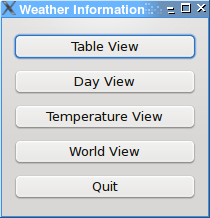
\includegraphics[width=7cm]{mainwidget.png}
\end{center}

\section{Die Tabellenansicht}
Die Tabellenansicht zeigt eine \"Ubersicht aller verf\"ugbaren Orte und das
Wetter an diesen innerhalb der n\"achsten 5 Tage.

\begin{center}
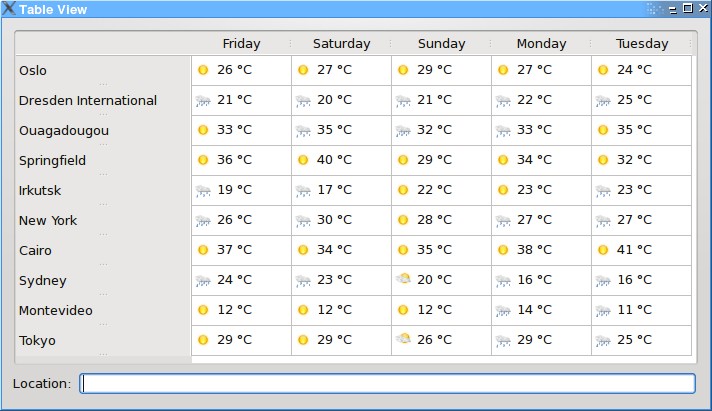
\includegraphics[width=14cm]{tableview.png}
\end{center}

Die Auswahl der angezeigten Orte kann vom Benutzer durch Eingabe eines
Namenfilters eingeschr\"ankt werden.

\begin{center}
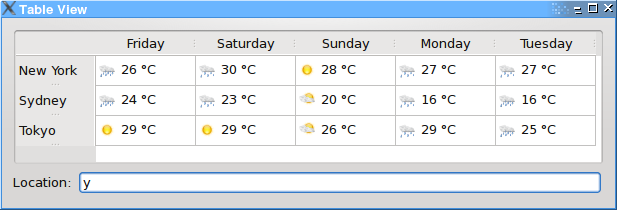
\includegraphics[width=14cm]{tableview_filtered.png}
\end{center}

Die Temperatur eines Ortes an einem Tag kann durch einen Doppelclick auf
die entsprechende Tabellenzelle und Eingabe des neuen Temperaturwertes
ge\"andert werden.

\section{Die Ortsansicht}
Die Ortsansicht zeigt die Wetterinformationen f\"ur einen bestimmten Ort
und Tag an. Der Benutzer kann Ort und Tag selbst ausw\"ahlen.

\begin{center}
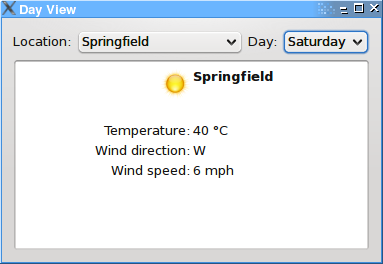
\includegraphics[width=14cm]{dayview.png}
\end{center}

\section{Die Temperaturansicht}
Die Temperaturansicht zeigt den Temperaturverlauf der n\"achsten 5 Tage
f\"ur einen bestimmten Ort an, welcher vom Benutzer selbst ausgew\"ahlt
werden kann.

\begin{center}
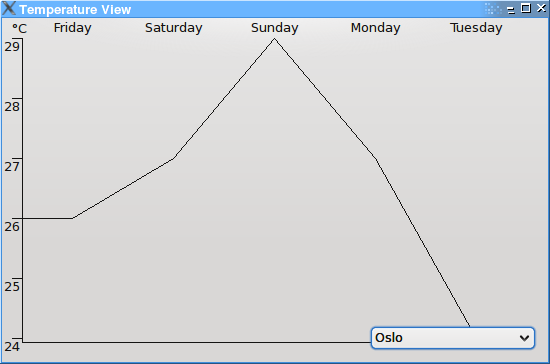
\includegraphics[width=14cm]{temperatureview.png}
\end{center}

\section{Die Weltansicht}
Die Weltansicht zeigt die Wetterbedingungen f\"ur einen bestimmten Tag
in allen verf\"ugbaren St\"adten an. Der Benutzer kann den Tag selbst
ausw\"ahlen.

\begin{center}
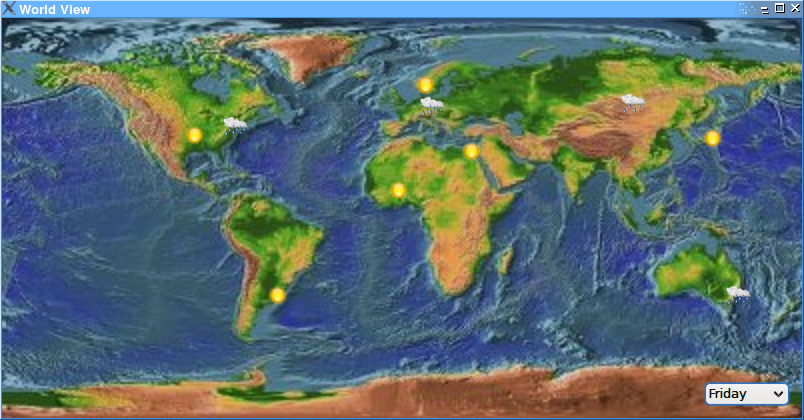
\includegraphics[width=14cm]{worldview.png}
\end{center}

\end{document}
